%%%%%%%%%%%%%%%%%%%%%%%%%%%%%%%%%%%%%%%%%
% Structured General Purpose Assignment
% LaTeX Template
%
% This template has been downloaded from:
% http://www.latextemplates.com
%
% Original author:
% Ted Pavlic (http://www.tedpavlic.com)
%
% Note:
% The \lipsum[#] commands throughout this template generate dummy text
% to fill the template out. These commands should all be removed when 
% writing assignment content.
%
%%%%%%%%%%%%%%%%%%%%%%%%%%%%%%%%%%%%%%%%%

%----------------------------------------------------------------------------------------
%	PACKAGES AND OTHER DOCUMENT CONFIGURATIONS
%----------------------------------------------------------------------------------------

\documentclass{article}

\usepackage{fancyhdr} % Required for custom headers
\usepackage{lastpage} % Required to determine the last page for the footer
\usepackage{extramarks} % Required for headers and footers
%\usepackage{graphicx} % Required to insert images
\usepackage{lipsum} % Used for inserting dummy 'Lorem ipsum' text into the template

\sloppy
\makeindex

\usepackage[latin1]{inputenc}
\usepackage{amsmath, marvosym} % Mathematik
\usepackage{harvard} %for harvard style citation, keep this position before url package
\usepackage{times, url, geometry, amssymb, booktabs}
\usepackage{hyperref} %Hyperlinks zw. Textstellen
\usepackage[pdftex]{graphicx} %pdf figures
\usepackage{subfig} %multi-figures
\usepackage{listings} %code listings
\usepackage{multirow} %for multi-row tables
\usepackage{color} %needed for listings

%directory for graphics
\graphicspath{{gfx/}}

% Margins
\topmargin=-0.45in
\evensidemargin=0in
\oddsidemargin=0in
\textwidth=6.5in
\textheight=9.0in
\headsep=0.25in 

\linespread{1.1} % Line spacing

% Set up the header and footer
\pagestyle{fancy}
\lhead{\hmwkAuthorName} % Top left header
%\chead{\hmwkClass\ (\hmwkClassInstructor\ \hmwkClassTime): \hmwkTitle} % Top center header
%\rhead{\firstxmark} % Top right header
\rhead{Problem Set 4} % Top right header
%\lfoot{\lastxmark} % Bottom left footer
\cfoot{} % Bottom center footer
\rfoot{Page\ \thepage\ of\ \pageref{LastPage}} % Bottom right footer
\renewcommand\headrulewidth{0.4pt} % Size of the header rule
\renewcommand\footrulewidth{0.4pt} % Size of the footer rule

\setlength\parindent{0pt} % Removes all indentation from paragraphs

%----------------------------------------------------------------------------------------
%	DOCUMENT STRUCTURE COMMANDS
%	Skip this unless you know what you're doing
%----------------------------------------------------------------------------------------

% Header and footer for when a page split occurs within a problem environment
\newcommand{\enterProblemHeader}[1]{
\nobreak\extramarks{#1}{#1 continued on next page\ldots}\nobreak
\nobreak\extramarks{#1 (continued)}{#1 continued on next page\ldots}\nobreak
}

% Header and footer for when a page split occurs between problem environments
\newcommand{\exitProblemHeader}[1]{
\nobreak\extramarks{#1 (continued)}{#1 continued on next page\ldots}\nobreak
\nobreak\extramarks{#1}{}\nobreak
}

\setcounter{secnumdepth}{0} % Removes default section numbers
\newcounter{homeworkProblemCounter} % Creates a counter to keep track of the number of problems

\newcommand{\homeworkProblemName}{}
\newenvironment{homeworkProblem}[1][Part \arabic{homeworkProblemCounter}: Implementation]{ % Makes a new environment called homeworkProblem which takes 1 argument (custom name) but the default is "Problem #"
\stepcounter{homeworkProblemCounter} % Increase counter for number of problems
\renewcommand{\homeworkProblemName}{#1} % Assign \homeworkProblemName the name of the problem
\section{\homeworkProblemName} % Make a section in the document with the custom problem count
\enterProblemHeader{\homeworkProblemName} % Header and footer within the environment
}{
\exitProblemHeader{\homeworkProblemName} % Header and footer after the environment
}

\newcommand{\problemAnswer}[1]{ % Defines the problem answer command with the content as the only argument
\noindent\framebox[\columnwidth][c]{\begin{minipage}{0.98\columnwidth}#1\end{minipage}} % Makes the box around the problem answer and puts the content inside
}

\newcommand{\homeworkSectionName}{}
\newenvironment{homeworkSection}[1]{ % New environment for sections within homework problems, takes 1 argument - the name of the section
\renewcommand{\homeworkSectionName}{#1} % Assign \homeworkSectionName to the name of the section from the environment argument
\subsection{\homeworkSectionName} % Make a subsection with the custom name of the subsection
\enterProblemHeader{\homeworkProblemName\ [\homeworkSectionName]} % Header and footer within the environment
}{
\enterProblemHeader{\homeworkProblemName} % Header and footer after the environment
}
   
%----------------------------------------------------------------------------------------
%	NAME AND CLASS SECTION
%----------------------------------------------------------------------------------------

\newcommand{\hmwkTitle}{Assignment\ \#1} % Assignment title
\newcommand{\hmwkDueDate}{Monday,\ January\ 1,\ 2012} % Due date
\newcommand{\hmwkClass}{BIO\ 101} % Course/class
\newcommand{\hmwkClassTime}{10:30am} % Class/lecture time
\newcommand{\hmwkClassInstructor}{Jones} % Teacher/lecturer
\newcommand{\hmwkAuthorName}{Budi Yanto} % Your name

%----------------------------------------------------------------------------------------
%	TITLE PAGE
%----------------------------------------------------------------------------------------

%\title{
%\vspace{2in}
%\textmd{\textbf{\hmwkClass:\ \hmwkTitle}}\\
%\normalsize\vspace{0.1in}\small{Due\ on\ \hmwkDueDate}\\
%\vspace{0.1in}\large{\textit{\hmwkClassInstructor\ \hmwkClassTime}}
%\vspace{3in}
%}

%\author{\textbf{\hmwkAuthorName}}
%\date{} % Insert date here if you want it to appear below your name

%----------------------------------------------------------------------------------------

\begin{document}

%\maketitle
%############################################################################
%########################### Change This ####################################
%############################################################################
%put your title here
\newcommand{\trtitle}{Problem Set 4: Support Vector Machines}
%replace with "Bachelor Thesis", "Master Thesis" or "Diplomarbeit"
\newcommand{\trtype}{Report Machine Learning Lab Course}
%your name
\newcommand{\trauthor}{Budi Yanto}
% your matrikelnummer
\newcommand{\trmatrikelnummer}{308819}
\newcommand{\tremail}{budiyanto@mailbox.tu-berlin.de}
%supevisor
%\newcommand{\trbetreuerA}{Daniel Bratz}
%\newcommand{\trbetreuerB}{Dipl.-Ing. Jo\"{e}l Chinnow}
%estimator 1
\newcommand{\trguta}{Daniel Bartz}
%estimator two
\newcommand{\trgutb}{Felix Brockherde}
\newcommand{\trdate}{\today}

%############################################################################
%########################### DO NOT touch this, unless you need to ##########
%############################################################################
\thispagestyle{empty}
%head line logo + tub + logo
\begin{tabular}{lcc}
\includegraphics[width=0.15\textwidth]{template/TUBerlin_Logo_rot_hell}& \hspace{1.1cm} Technische Universit{\"a}t Berlin& \hspace{1.2cm} 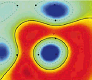
\includegraphics[width=0.15\textwidth]{template/ml_logo}\\
\end{tabular}
%draw a line
\rule{\textwidth}{0.4pt}
%aub: remove this on final submission
%\begin{center}
%DOCUMENT BUILD DATE: \today\\%
%add your status here, e.g. First Draft for Supervizor etc.
%DOCUMENT STATUS: Beta
%\end{center}

%vertical space
\vspace{2.5cm}
\begin{center}
%replace this
  \textbf{\LARGE \trtitle}
\end{center}
\vspace{2cm}

\begin{center}
  \textbf{\trtype} \\
  Fachgebiet Maschinelles Lernen\\
  Prof.\ Dr.\ Klaus-Robert M�ller \\
  Fakult�t IV Elektrotechnik und Informatik \\
  Technische Universit�t Berlin \\[0.5cm]
  submitted by \\
  \textbf{\trauthor}
\end{center}

\vspace{1cm}


\begin{center}
\begin{tabular}{ll}
Instructor:& \trguta\\
& \trgutb\\
\end{tabular}
\end{center}

\vfill

\begin{tabular}{l}
Matrikelnummer:  \trmatrikelnummer \\
Email: \tremail \\
\end{tabular}

\rule{\textwidth}{0.4pt}

\clearpage
\newpage
%----------------------------------------------------------------------------------------
%	TABLE OF CONTENTS
%----------------------------------------------------------------------------------------

%\setcounter{tocdepth}{1} % Uncomment this line if you don't want subsections listed in the ToC

%\newpage
%\tableofcontents
%\newpage

%----------------------------------------------------------------------------------------
%	PROBLEM 1
%----------------------------------------------------------------------------------------

% To have just one problem per page, simply put a \clearpage after each problem

\begin{homeworkProblem}[Part \arabic{homeworkProblemCounter}: Implementation]

In this part, the pseudocode of the SMO from the handbook and the class \textit{svm\_qp} that solves the SVM dual optimization problem as a quadratic programming problem were implemented. Furthermore, a function to plot the SVM 2D was also implemented.

%--------------------------------------------

\begin{homeworkSection}{Assignment 1: SMO}

The SVM SMO should be implemented in this assignment. The implementation was pretty straight forward and the pseudocode in the handbook was really helpful to implement the SMO. All of the tests provided for this assignment were passed. Figure~\ref{fig:svmSMOTest} shows the 2D plot of the SVM SMO applied to the test data.

\begin{figure}[h!]
	\centering
 	\subfloat[SVM SMO applied to the test data]{
     	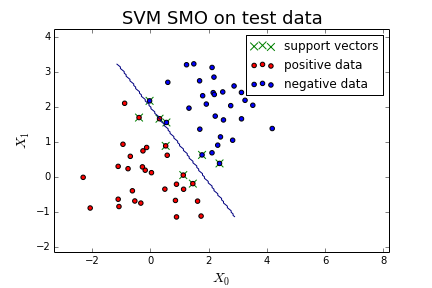
\includegraphics[width=0.5\textwidth]{SVM_SMO_Test}
		\label{fig:svmSMOTest}
	}
    %~
	\subfloat[SVM QP applied to the test data]{
    		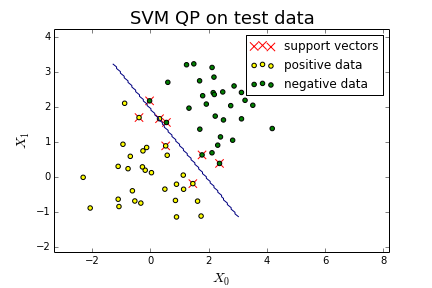
\includegraphics[width=0.5\textwidth]{SVM_QP_Test} % Example image
		\label{fig:svmQPTest}
	}
	\caption{SVM SMO and SVM SMO applied to the test data}
\end{figure}

\end{homeworkSection}

%--------------------------------------------

\begin{homeworkSection}{Assignment 2: Plot SVM 2D}

This function was implemented to plot the 2D data points and its corresponding support vectors. In addition, the separating hyperplane is also plotted. The positive data points are drawn as yellow circles whereas the negative data points are drawn as green circles. The support vectors on the other hand are drawn as red crosses.

\end{homeworkSection}

%--------------------------------------------

\begin{homeworkSection}{Assignment 3: SVM QP}

In this assignment, the SVM dual optimization problem should be solved as a quadratic programming problem. The method \textit{cvxopt.solvers.qp} from the package \textit{cvxopt} was used to solve the QP problem. It was pretty straight forward to implement this method. We have to figure out how to reformulate the SVM dual optimization problem to the form of QP problem. The most difficult part in this assignment was actually trying to figure out how to calculate the bias \textit{b}. Figure~\ref{fig:svmQPTest} shows the 2D plot of the SVM QP applied to the test data.

\end{homeworkSection}

%--------------------------------------------

\end{homeworkProblem}

%\clearpage
\newpage
%----------------------------------------------------------------------------------------
%	PROBLEM 2
%----------------------------------------------------------------------------------------

\begin{homeworkProblem}[Part \arabic{homeworkProblemCounter}: Application] 

In this part, the SVM SMO implementation should be applied to the \textit{Easy\_2D} and \textit{UCI Iris} datasets. In addition to that, the running time of the \textit{svm\_qp} implementation should be compared to the properly implemented SMO routine \textit{svm\_sklearn}.

%--------------------------------------------

\begin{homeworkSection}{Assignment 4: Easy\_2D Dataset} % Section within problem

In this assignment, the Cross-Validation should be used to find the optimal parameters $C$ and $\sigma$ for a Gaussian kernel. Table~\ref{crossValdidationParameters} shows the parameters used to run the Cross-Validation whereas Table~\ref{optimalParametersCV} shows the optimal parameters and properties obtained by the Cross-Validation. The result of the SVM that run using the optimal parameters is depicted in Figure~\ref{fig:svmSMOEasy2D}. The SVM SMO obtained 55 support vectors from total 100 data points. The SVM SMO with the optimal parameters was also run on the test data from the easy\_2D dataset, and got 0.01 loss which is actually quite low. It got 0.07 loss when it was run to predict the true data.

\begin{table}[h!]
	\centering
	\begin{tabular}{l*{6}{c}r}
		\textbf{Kernel}    & \textbf{Kernel Parameters} & \textbf{Regularization} & \textbf{nRepetitions} & \textbf{nFolds} \\
		\hline
		Gaussian & np.logspace(-2,2,10) & np.logspace(-2,2,10) & 2 & 10  \\
		
	\end{tabular}
	\caption{Parameters used to run the Cross-Validation}
	\label{crossValdidationParameters}
\end{table}

\begin{table}[h!]
	\centering
	\begin{tabular}{l*{6}{c}r}
		\textbf{Kernel}    & \textbf{Kernel Parameters} & \textbf{Regularization} & \textbf{Cvloss} & \textbf{Loss on easy\_Xte} \\
		\hline
		Gaussian & 0.21544 & 1.6681 & 0.1 & 0.01  \\
		
	\end{tabular}
	\caption{Optimal parameters and properties obtained by the Cross-Validation}
	\label{optimalParametersCV}
\end{table}

\begin{figure}[h!]
	\centering
	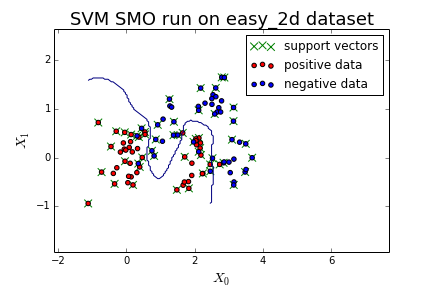
\includegraphics[width=0.75\columnwidth]{SVM_SMO_Easy_2D} % Example image
	\caption{SVM SMO applied to the \textit{easy\_2D} dataset}
	\label{fig:svmSMOEasy2D}
\end{figure}

Now the SVM should be trained with $C$ and $\sigma$ that obviously underfit and overfit the data. As $C$ increases, the SVM will overfit the data, since it tries to classify all data correctly. On the other hand, as $C$ decreases, it will underfit the data. An opposite behaviour applies to $\sigma$. As $\sigma$ increases, it will underfit the data, whereas as $\sigma$ decreases, it will overfit the data. Figure~\ref{fig:lossVariousC} and Figure~\ref{fig:lossVariousSigma} show this behaviour, as we can see from the loss values that were obtained by varying $C$ and $\sigma$, by holding the other parameter fixed. The optimal value of $C$, which was obtained by the Cross-Validation, was used as $\sigma$ was varied and the optimal value of $\sigma$ was used as $C$ was varied. Figure~\ref{fig:underfitEasy2D} and Figure~\ref{fig:overfitEasy2D} depict the SVM SMO that underfit and overfit the data, respectively. By varying the bias parameter $b$, the ROC-Curve for the optimal $C$ and $\sigma$ was plotted, as shown in Figure~\ref{fig:rocEasy2D}

\begin{figure}[h!]
	\centering
 	\subfloat[Loss values with various $C$ and $\sigma=0.2154$]{
     	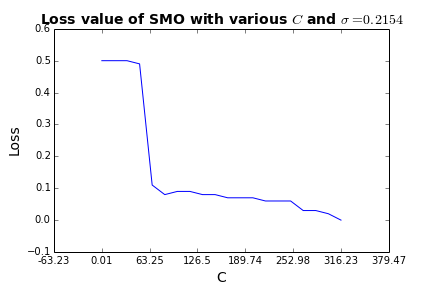
\includegraphics[width=0.5\textwidth]{loss_various_c}
		\label{fig:lossVariousC}
	}
    %~
	\subfloat[Loss values with various $\sigma$ and $C=1.6681$]{
    		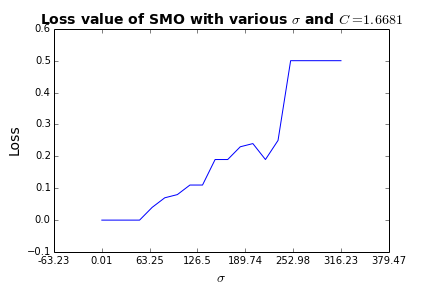
\includegraphics[width=0.5\textwidth]{loss_various_sigma}
		\label{fig:lossVariousSigma}
	}
	\caption{Loss values with various $C$ and $\sigma$}
\end{figure}

\begin{figure}[h!]
	\centering
 	\subfloat[Underfitting with $C=0.01$ and $\sigma=300$]{
     	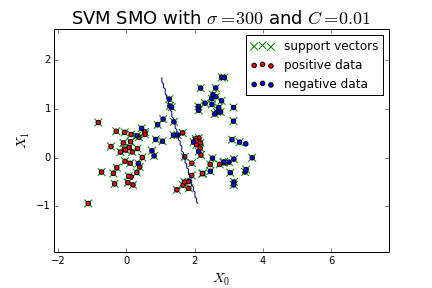
\includegraphics[width=0.5\textwidth]{underfit_easy2d}
		\label{fig:underfitEasy2D}
	}
    %~
	\subfloat[Overfitting with $\sigma=0.01$ and $C=300$]{
    		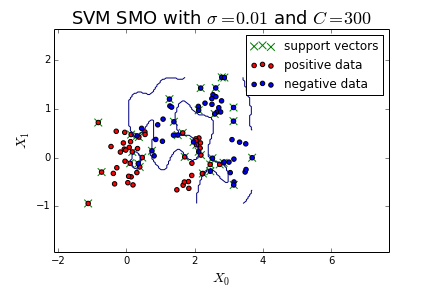
\includegraphics[width=0.5\textwidth]{overfit_easy2d}
		\label{fig:overfitEasy2D}
	}
	\caption{Underfitting and overfitting on the \textit{easy\_2D} dataset}
\end{figure}

\begin{figure}[h!]
	\centering
	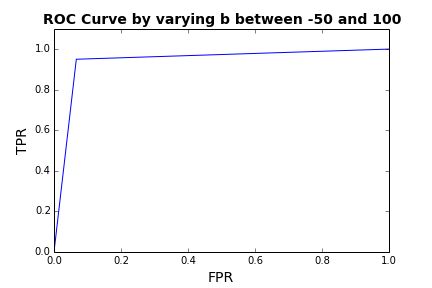
\includegraphics[width=0.75\columnwidth]{ROC_Easy2D}
	\caption{ROC-Curve by varying bias $b$ between -50 and 100}
	\label{fig:rocEasy2D}
\end{figure}

\end{homeworkSection}

%--------------------------------------------

\begin{homeworkSection}{Assignment 5: Sklearn} % Section within problem

Not finished yet - TODO

\end{homeworkSection}

%--------------------------------------------

\begin{homeworkSection}{Assignment 6: UCI Iris Dataset} % Section within problem

Not finished yet - TODO

\end{homeworkSection}

%--------------------------------------------

\end{homeworkProblem}

%----------------------------------------------------------------------------------------

\end{document}
